\chapter{Multiple Discrete Random Variables}
\label{chapter:RandomVectorsDiscrete}

Thus far, our treatment of probability has been focused on single random variables.
It is often convenient or required to model stochastic phenomena using multiple random variables.
In this section, we extend some of the concepts developed for single random variables to multiple random variables.
We center our exposition of random vectors around the simplest case, pairs of random variables.


\section{Joint Probability Mass Functions}

Consider two discrete random variables $X$ and $Y$ associated with a single experiment.
The random pair $(X, Y)$ is characterized by the \emph{joint probability mass function} of $X$ and $Y$, which we denote by $p_{X,Y}(\cdot,\cdot)$. \index{Joint probability mass function}
If $x$ is a possible value of $X$ and $y$ is a possible value of $Y$, then the probability mass function of $(x, y)$ is denoted by
\begin{equation*}
\begin{split}
p_{X,Y} (x, y) &= \Pr ( \{ X = x \} \cap \{ Y = y \} ) \\
&= \Pr ( X = x, Y = y ).
\end{split}
\end{equation*}
Note the similarity between the definition of the joint PMF and \eqref{equation:PMF}.

\begin{figure}[ht]
\begin{center}
\begin{psfrags}
\psfrag{1}[c]{$1$}
\psfrag{2}[c]{$2$}
\psfrag{3}[c]{$3$}
\psfrag{4}[c]{$4$}
\psfrag{5}[c]{$5$}
\psfrag{6}[c]{$6$}
\psfrag{7}[c]{$7$}
\psfrag{S}[l]{Sample Space}
\psfrag{R}[c]{$\RealNumbers$}
\psfrag{X}[c]{$X$}
\psfrag{Y}[c]{$Y$}
\psfrag{P}[c]{$(X,Y)$}
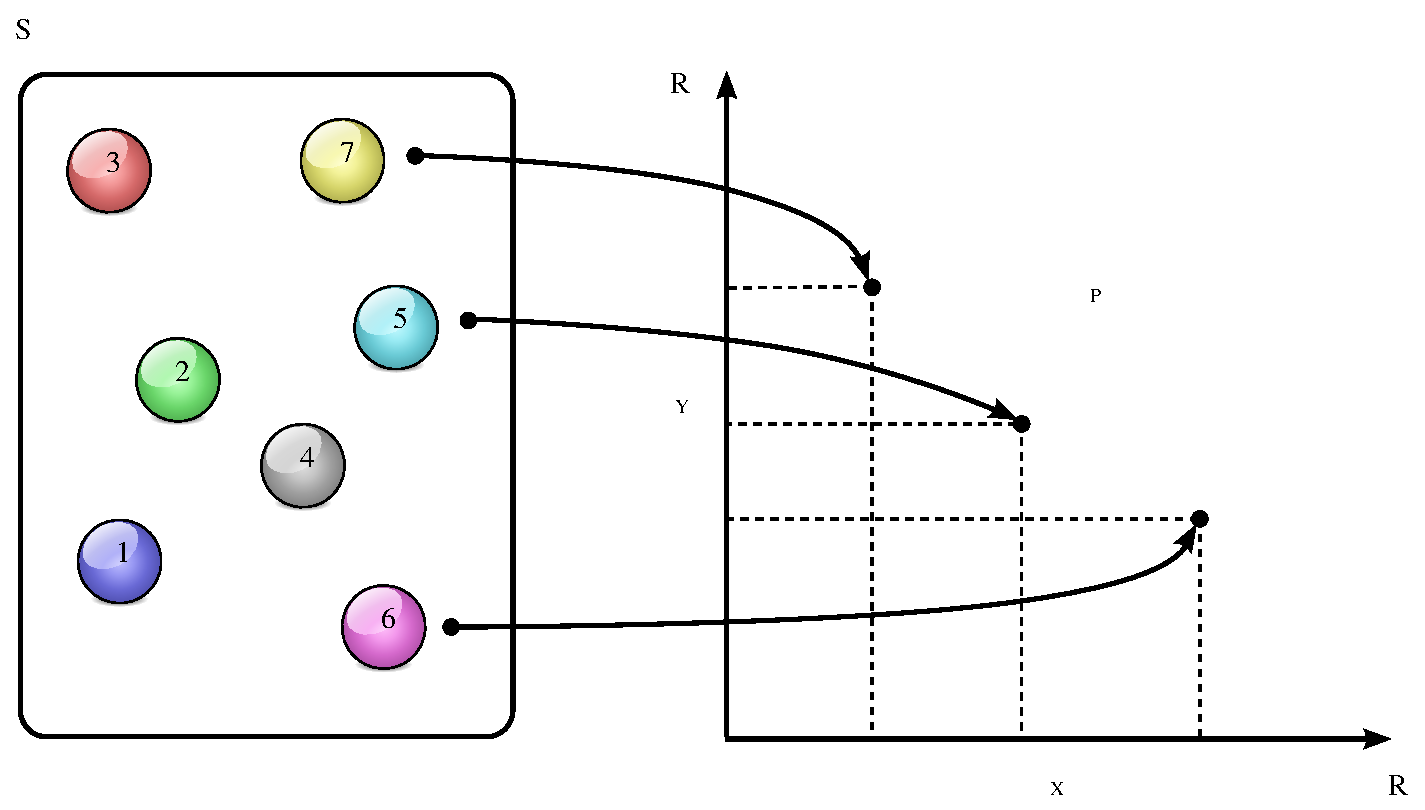
\includegraphics[height=5.20cm]{Figures/7Chapter/prv}
\end{psfrags}
\caption{The random pair $(X, Y)$ maps every outcome contained in the sample space to a vector in $\RealNumbers^2$.}
\end{center}
\end{figure}

Suppose that $S$ is a subset of $X(\Omega) \times Y(\Omega)$.
We can express the probability of $S$ as
\begin{equation*}
\begin{split}
\Pr (S) &= \Pr (\{ \omega \in \Omega | (X(\omega), Y(\omega)) \in S \}) \\
&= \sum_{(x,y) \in S} p_{X,Y} (x, y) .
\end{split}
\end{equation*}
In particular, we have
\begin{equation*}
\sum_{x \in X(\Omega)} \sum_{y \in Y(\Omega)} p_{X,Y} (x, y) = 1.
\end{equation*}

To further distinguish between the joint PMF of $(X, Y)$ and the individual PMFs $p_X (\cdot)$ and $p_Y (\cdot)$, we occasionally refer to the latter as \emph{marginal probability mass functions}. \index{Probability mass function (PMF)} \index{Marginal probability mass function}
We can compute the marginal PMFs of $X$ and $Y$ from the joint PMF $p_{X,Y}(\cdot,\cdot)$ using the formulas
\begin{align*}
p_X (x) &= \sum_{y \in Y(\Omega)} p_{X,Y} (x,y), \\
p_Y (y) &= \sum_{x \in X(\Omega)} p_{X,Y} (x,y).
\end{align*}
On the other hand, knowledge of the marginal distributions $p_X (\cdot)$ and $p_Y (\cdot)$ is not enough to obtain a complete description of the joint PMF $p_{X,Y} (\cdot,\cdot)$.
This fact is illustrated in Examples~\ref{example:JointPMFwoReplacement}~\&~\ref{example:JointPMFwithReplacement}.

\begin{example} \label{example:JointPMFwoReplacement}
An urn contains three balls numbered one, two and three.
A random experiment consists of drawing two balls from the urn, without replacement.
The number appearing on the first ball is a random variable, which we denote by $X$.
Similarly, we refer to the number inscribed on the second ball as $Y$.
The joint PMF of $X$ and $Y$ is specified in table form below,
\begin{center}
\begin{tabular}{|c|c|c|c|}
\hline
$p_{X,Y} (x,y)$ & $1$ & $2$ & $3$ \\
\hline
$1$ & $0$ & $1/6$ & $1/6$ \\
\hline
$2$ & $1/6$ & $0$ & $1/6$ \\
\hline
$3$ & $1/6$ & $1/6$ & $0$ \\
\hline
\end{tabular} .
\end{center}
We can compute the marginal PMF of $X$ as
\begin{equation*}
p_X (x) = \sum_{y \in Y(\Omega)} p_{X,Y} (x,y)
= \frac{1}{6} + \frac{1}{6} = \frac{1}{3},
\end{equation*}
where $x \in \{1, 2, 3 \}$.
Likewise, the marginal PMF of $Y$ is given by
\begin{equation*}
p_Y (y) = \left\{ \begin{array}{ll}
1/3, & \text{if }y \in \{ 1, 2, 3 \} \\
0, & \text{otherwise} .
\end{array} \right.
\end{equation*}
\end{example}

\begin{example} \label{example:JointPMFwithReplacement}
Again, suppose that an urn contains three balls numbered one, two and three.
This time the random experiment consists of drawing two balls from the urn with replacement.
We use $X$ and $Y$ to denote the numbers appearing on the first and second balls, respectively.
The joint PMF of $X$ and $Y$ becomes
\begin{center}
\begin{tabular}{|c|c|c|c|}
\hline
$p_{X,Y} (x,y)$ & $1$ & $2$ & $3$ \\
\hline
$1$ & $1/9$ & $1/9$ & $1/9$ \\
\hline
$2$ & $1/9$ & $1/9$ & $1/9$ \\
\hline
$3$ & $1/9$ & $1/9$ & $1/9$ \\
\hline
\end{tabular} .
\end{center}
The marginal distributions of $X$ and $Y$ are the same as in Example~\ref{example:JointPMFwoReplacement};
however, the joint PMFs differ.
\end{example}


\section{Functions and Expectations}

Let $X$ and $Y$ be two random variables with joint PMF $p_{X,Y} (\cdot, \cdot)$.
Consider a third random variable defined by $V = g(X,Y)$, where $g (\cdot, \cdot)$ is a real-valued function.
We can obtain the PMF of $V$ by computing
\begin{equation} \label{equation:PMFSumDiscrete}
p_V (v)
= \sum_{\{ (x,y) | g(x,y) = v \}} p_{X,Y} (x, y).
\end{equation}
This equation is the analog of \eqref{equation:FunctionPMF} for pairs of random variables.

\begin{figure}[ht]
\begin{center}
\begin{psfrags}
\psfrag{1}[c]{$1$}
\psfrag{2}[c]{$2$}
\psfrag{3}[c]{$3$}
\psfrag{4}[c]{$4$}
\psfrag{5}[c]{$5$}
\psfrag{S}[l]{Sample Space}
\psfrag{R}[c]{$\RealNumbers$}
\psfrag{X}[c]{$X$}
\psfrag{Y}[c]{$Y$}
\psfrag{Z}[c]{$V$}
\psfrag{g}[c]{$V = g(X,Y)$}

\includegraphics[width=11cm]{Figures/7Chapter/vfcn}
\end{psfrags}
\caption{A real-valued function of two random variables, $X$ and $Y$, is also a random variable.
Above, $V = g(X, Y)$ maps elements of the sample space to real numbers.}
\end{center}
\end{figure}

\begin{example} \label{example:SumDice1}
Two dice, a blue die and a red one, are rolled simultaneously.
The random variable $X$ represents the number of dots that appears on the top face of the blue die, whereas $Y$ denotes the number of dots on the red die.
We can form a random variable $U$ that describes the sum of these two dice, $U = X + Y$.

The lowest possible value for $U$ is two, and its maximum value is twelve.
The PMF of $U$, as calculated using \eqref{equation:PMFSumDiscrete}, appears in table form below
\begin{center}
\begin{tabular}{|c|c|c|c|c|c|c|}
\hline
$k$ & $2, 12$ & $3, 11$ & $4, 10$ & $5, 9$ & $6, 8$ & $7$ \\
\hline
$p_U (k)$ & $1/36$ & $1/18$ & $1/12$ & $1/9$ & $5/36$ & $1/6$ \\
\hline
\end{tabular}
\end{center}
\end{example}

The definition of the expectation operator can be extended to multiple random variables.
In particular, the expected value of $g(X,Y)$ is obtained by computing
\begin{equation} \label{equation:ExpectationMultipleRV}
\Expect [g(X,Y)] = \sum_{x \in X(\Omega)} \sum_{y \in Y(\Omega)} g(x,y) p_{X,Y} (x,y) .
\end{equation}

\begin{example}
An urn contains three balls numbered one, two and three.
Two balls are selected from the urn at random, without replacement.
We employ $X$ and $Y$ to represent the numbers on the first and second balls, respectively.
We wish to compute the expected value of the function $X + Y$.

Using \eqref{equation:ExpectationMultipleRV}, we compute the expectation of $g(X,Y) = X + Y$ as
\begin{equation*}
\begin{split}
\Expect [g(X,Y)] &= \Expect [X + Y] \\
&= \sum_{x \in X(\Omega)} \sum_{y \in Y(\Omega)} (x + y) p_{X,Y} (x,y) \\
&= \sum_{x \in X(\Omega)} x p_X (x) + \sum_{y \in Y(\Omega)} y p_Y (y)
= 4.
\end{split}
\end{equation*}
The expected value of $X + Y$ is four.
\end{example}


\section{Conditional Random Variables}
\label{section:ConditionalRandomVariables}

Many events of practical interest are dependent.
That is, knowledge about event $A$ may provide partial information about the realization of event $B$.
This inter-dependence is captured by the concept of conditioning, which was first discussed in Chapter~\ref{chapter:ConditionalProbability}.
In this section, we extend the concept of conditioning to multiple random variables.
We study the probability of events concerning random variable $Y$ given that some information about random variable $X$ is available.

Let $X$ and $Y$ be two random variables associated with a same experiment.
The \emph{conditional probability mass function} of $Y$ given $X = x$, which we write $p_{Y|X} (\cdot | \cdot)$, is defined by \index{Conditional probability mass function}
\begin{equation*}
\begin{split}
p_{Y|X} (y|x) &= \Pr ( Y = y | X = x) \\
&= \frac{\Pr (\{Y = y\} \cap \{ X = x \})}{\Pr (X = x)} \\
&= \frac{ p_{X,Y} (x,y) }{p_X(x)},
\end{split}
\end{equation*}
provided that $p_X (x) \neq 0$.
Note that conditioning on $X = x$ is not possible when $p_X (x)$ vanishes, as it has no relevant meaning.
This is similar to conditional probabilities being only defined for conditional events with non-zero probabilities.

Let $x$ be fixed with $p_X (x) > 0$.
The conditional PMF introduced above is a valid PMF since it is nonnegative and
\begin{equation*}
\begin{split}
\sum_{y \in Y(\Omega)} p_{Y|X} (y|x)
&= \sum_{y \in Y(\Omega)} \frac{p_{X,Y} (x,y)}{p_X (x)} \\
&= \frac{1}{p_X (x)} \sum_{y \in Y(\Omega)} p_{X,Y} (x,y) = 1.
\end{split}
\end{equation*}
The probability that $Y$ belongs to $S$, given $X = x$, is obtained by summing the conditional probability $p_{Y|X} (\cdot | \cdot)$ over all outcomes included in $S$,
\begin{equation*}
\Pr (Y \in S | X = x) = \sum_{y \in S} p_{Y|X} (y | x) .
\end{equation*}

\begin{example}[Hypergeometric Random Variable]
A wireless communication channel is employed to transmit a data packet that contains a total of $m$ bits.
The first $n$ bits of this message are dedicated to the packet header, which stores very sensitive information.
The wireless connection is unreliable; every transmitted bit is received properly with probability $1-p$ and erased with probability $p$, independently of other bits.
We wish to derive the conditional probability distribution of the number of erasures located in the header, given that the total number of corrupted bits in the packet is equal to $e$.

Let $H$ represent the number of erasures in the header, and denote the number of corrupted bits in the entire message by $C$.
The conditional probability mass function of $H$ given $C = c$ is equal to
\begin{equation*}
\begin{split}
p_{H|C} (h|c) &= \frac{p_{H,C} (h,c)}{p_H (h)} \\
&= \frac{\binom{n}{h} (1-p)^{n-h} p^h
\binom{m-n}{c-h} (1-p)^{(m-n)-(c-h)} p^{c - h}}{\binom{m}{c} (1-p)^{m-c} p^c} \\
&= \frac{\binom{n}{h} \binom{m-n}{c-h}}{\binom{m}{c}} ,
\end{split}
\end{equation*}
where $h = 0, 1, \ldots \min \{ e, m \}$.
Clearly, the conditioning affects the probability distribution of the number of corrupted bits in the header.
In general, a random variable with such a distribution is known as a \emph{hypergeometric random variable}. \index{Hypergeometric random variable}
\end{example}

%\begin{example}
%Suppose that an urn contains three balls numbered one, two and three.
%Two balls are drawn from this urn without replacement.
%We wish to find the probability that the number on the second ball is odd.
%We also wish to identify the probability that the second ball is odd given that the number on the first ball is a three.
%
%The probability that the number on the second ball is odd is given by the marginal distribution of the second  drawing, which was derived in Example~\ref{example:JointPMFwoReplacement}.
%In the notation of that example, we have
%\begin{equation*}
%\Pr (Y \in \{1, 3\})
%= p_Y (1) + p_Y (3)
%= \frac{1}{3} + \frac{1}{3}
%= \frac{2}{3} .
%\end{equation*}
%To compute the probability that the second ball is odd conditioned on the first ball being a three, we use the joint PMF obtained in Example~\ref{example:JointPMFwoReplacement},
%\begin{equation*}
%\begin{split}
%\Pr ( Y \in \{ 1, 3 \} | X = 3)
%&= p_{Y|X}(1|3) + p_{Y|X}(3|3) \\
%&= \frac{p_{X,Y}(1,3)}{p_X (3)} + \frac{p_{X,Y}(3,3)}{p_X (3)} \\
%&= \frac{1/6}{1/3} + \frac{0}{1/3} = \frac{1}{2} .
%\end{split}
%\end{equation*}
%The conditioning affects the probability of the second number drawn being odd.
%\end{example}

The definition of conditional PMF can be rearranged to obtain a convenient formula to calculate the joint distribution of $X$ and $Y$, namely
\begin{equation*}
p_{X,Y} (x,y) = p_{Y|X} (y|x) p_X (x)
 = p_{X|Y} (x|y) p_Y (y) .
\end{equation*}
This formula can be use to compute the joint PMF of $X$ and $Y$ sequentially.

\begin{example}[Splitting Property of Poisson PMF]
A digital communication system sends out either a one with probability $p$ or a zero with probability $1 - p$, independently of previous transmissions.
The number of transmitted binary digits within a given time interval has a Poisson PMF with parameter $\lambda$.
We wish to show that the number of ones sent in that same time interval has a Poisson PMF with parameter $p \lambda$.

Let $M$ denote the number of ones within the stipulated interval, $N$ be the number of zeros, and $K = M + N$ be the total number of bits sent during the same interval.
The number of ones given that the total number of transmissions is $k$ is given by
\begin{equation*}
p_{M|K} (m | k) = \binom{k}{m} p^m (1-p)^{k - m},
\quad m = 0, 1, \ldots, k.
\end{equation*}
The probability that $M$ is equal to $m$ is therefore equal to
\begin{equation*}
\begin{split}
p_{M} (m) &= \sum_{k = 0}^{\infty} p_{K,M} (k, m)
= \sum_{k = 0}^{\infty} p_{M|K} (m | k) p_K(k) \\
&= \sum_{k = m}^{\infty} \binom{k}{m} p^m (1-p)^{k - m}
\frac{\lambda^{k}}{k !} e^{-\lambda} \\
&= \sum_{u = 0}^{\infty} \binom{u+m}{m} p^m (1-p)^{u}
\frac{\lambda^{u+m}}{(u+m)!} e^{-\lambda} \\
&= \frac{(\lambda p)^m}{m!} e^{-\lambda}
\sum_{u = 0}^{\infty} \frac{( (1-p) \lambda)^{u}}{u!}
= \frac{(\lambda p)^m}{m!} e^{-p \lambda} .
\end{split}
\end{equation*}
Above, we have used the change of variables $k = u+m$.
We have also rearranged the sum into a familiar form, leveraging the fact that the summation of a Poisson PMF over all possible values is equal to one.
We can see that $M$ has a Poisson PMF with parameter $p \lambda$.
\end{example}


\subsection{Conditioning on Events}

It is also possible to define the conditional PMF of a random variable $X$, conditioned on an event $S$ where $\Pr (X \in S) > 0$.
Let $X$ be a random variable associated with a particular experiment, and let $S$ be a non-trivial event corresponding to this experiment.
The conditional PMF of $X$ given $S$ is defined by
\begin{equation} \label{equation:ConditionalEventPMF}
p_{X|S} (x) = \Pr (X = x | S)
= \frac{\Pr (\{X = x\} \cap S)}{\Pr (S)} .
\end{equation}
Note that the events $\{ \omega \in \Omega |  X(\omega) = x \}$ form a partition of $\Omega$ as $x$ ranges over all the values in $X (\Omega)$.
Using the total probability theorem, we gather that
\begin{equation*}
\sum_{x \in X(\Omega)} \Pr ( \{X = x\} \cap S) = \Pr (S)
\end{equation*}
and, consequently, we get
\begin{equation*}
\begin{split}
\sum_{x \in X(\Omega)} p_{X|S} (x)
&= \sum_{x \in X(\Omega)} \frac{\Pr (\{X = x\} \cap S)}{\Pr (S)} \\
&= \frac{\sum_{x \in X(\Omega)} \Pr (\{X = x\} \cap S)}{\Pr (S)}
=1 .
\end{split}
\end{equation*}
We conclude that $p_{X|S} (\cdot)$ is a valid PMF.

Another interpretation of \eqref{equation:ConditionalEventPMF} is the following.
Let $Y = \IndicatorFcn_S (\cdot)$ symbolize the indicator function of $S$, with
\begin{equation*}
\IndicatorFcn_S (\omega) = \begin{cases} 1, & \omega \in S\\
0, & \omega \notin S . \end{cases}
\end{equation*}
Then $p_{X|S} (x) = p_{X|Y} (x | 1)$.
In this sense, conditioning on an event is a special case of a conditional probability mass function.

\begin{example}
A data packet is sent to a destination over an unreliable wireless communication link.
Data is successfully decoded at the receiver with probability $p$, and the transmission fails with probability $(1-p)$, independently of previous trials.
When initial decoding fails, a retransmission is requested immediately.
However, if packet transmission fails $n$ consecutive times, then the data is dropped from the queue altogether, with no further transmission attempt.
Let $X$ denote the number of trials, and let $S$ be the event that the data packet is successfully transmitted.
We wish to compute the conditional PMF of $X$ given $S$.

First, we note that a successful transmission can happen at any of $n$ possible instants.
These outcomes being mutually exclusive, the probability of $S$ can be written as
\begin{equation*}
\Pr(S) = \sum_{k=1}^n (1-p)^{k-1} p = 1 - (1-p)^n .
\end{equation*}
Thus, the conditional PMF $p_{N|S} (\cdot)$ is equal to
\begin{equation*}
p_{N|S} (k) = \frac{ (1-p)^{k-1} p }{1 - (1-p)^n} ,
\end{equation*}
where $k = 1, 2, \ldots n$.
\end{example}


\section{Conditional Expectations}

The \emph{conditional expectation} of $Y$ given $X = x$ is simply the expectation of $Y$ with respect to the conditional PMF $p_{Y|X} (\cdot | x)$, \index{Conditional expectation}
\begin{equation*}
\Expect [Y | X = x ] = \sum_{y \in Y(\Omega)} y p_{Y|X} (y|x).
\end{equation*}
This conditional expectation can be viewed as a function of $x$,
\begin{equation*}
h(x) = \Expect [Y | X = x] .
\end{equation*}
It is therefore mathematically accurate and sometimes desirable to talk about the random variable $h (X) = \Expect [Y | X]$.
In particular, if $X$ and $Y$ are two random variables associated with an experiment, the outcome of this experiment determines the value of $X$, say $X = x$, which in turn yields the conditional expectation $h(x) = \Expect [Y | X = x]$.
From this point of view, the conditional expectation $\Expect [Y | X]$ is simply an instance of a random variable.

Not too surprisingly, the expectation of $\Expect [Y | X]$ is equal to $\Expect [Y]$, as evinced by the following derivation,
\begin{equation*}
\begin{split}
\Expect \left[ \Expect [Y | X] \right]
&= \sum_{x \in X(\Omega)} \Expect [Y | X = x] p_X (x) \\
&= \sum_{x \in X(\Omega)} \sum_{y \in Y(\Omega)} y p_{Y|X} (y|x) p_X (x) \\
&= \sum_{y \in Y(\Omega)} \sum_{x \in X(\Omega)} y p_{X,Y} (x, y) \\
%&= \sum_{y \in Y(\Omega)} y \sum_{x \in X(\Omega)} p_{X,Y} (x, y) \\
&= \sum_{y \in Y(\Omega)} y p_{Y} (y)
= \Expect [Y] .
\end{split}
\end{equation*}
Using a similar argument, it is straightforward to show that
\begin{equation*}
\Expect \left[ \Expect [g (Y) | X] \right] = \Expect [g(Y)] .
\end{equation*}

\begin{example}
An entrepreneur opens a small business that sells two kinds of beverages from the Brazos Soda Company, cherry soda and lemonade.
The number of bottles sold in an hour at the store is found to be a Poisson random variable with parameter $\lambda = 10$.
Every customer selects a cherry soda with probability $p$ and a lemonade with probability $(1 - p)$, independently of other customers.
We wish to find the conditional mean of the number of cherry sodas purchased in an hour given that ten beverages were sold to customers during this time period.

Let $B$ represent the number of bottles sold during an hour.
Similarly, let $C$ and $L$ be the number of cherry sodas and lemonades purchased during the same time interval, respectively.
We note that $B = C + L$.
The conditional PMF of $C$ given that the total number of beverages sold equals ten is
\begin{equation} \label{equation:ConditionalPoisson}
p_{C|B} (k | 10)
= \binom{10}{k} p^k (1-p)^{10-k} .
\end{equation}
This follows from the fact that every customer selects a cherry soda with probability $p$, independently of other customers.
The conditional mean is then seen to equal
\begin{equation*}
\Expect [ C | B=10] = \sum_{k=0}^{10}
k \binom{10}{k} p^k (1-p)^{10-k} = 10 p .
\end{equation*}
\end{example}

We can define the expectation of $X$ conditioned on event $S$ in an analogous fashion.
Let $S$ be an event such that $\Pr (S) > 0$.
The conditional expectation of $X$ given $S$ is
\begin{equation*}
\Expect [X | S] = \sum_{x \in X(\Omega)} x p_{X|S} (x) ,
\end{equation*}
where $p_{X|S} (\cdot)$ is defined in \eqref{equation:ConditionalEventPMF}.
Similarly, we have
\begin{equation*}
\Expect [g(X) | S] = \sum_{x \in X(\Omega)} g(x) p_{X|S} (x) ,
\end{equation*}

\begin{example}
Spring break is coming and a student decides to renew his shirt collection.
The number of shirts purchased by the student is a random variable denoted by $N$.
The PMF of this random variable is a geometric distribution with parameter $p = 0.5$.
Any one shirt costs \$10, \$20 or \$50 with respective probabilities 0.5, 0.3 and 0.2, independently of other shirts.
We wish to compute the expected amount of money spent by the student during his shopping spree.
Also, we wish to compute the expected amount of money disbursed given that the student buys at least five shirts.

Let $C_i$ be the cost of the $i$th shirt.
The total amount of money spent by the student, denoted by $T$, can be expressed as
\begin{equation*}
T = \sum_{i=1}^N C_i .
\end{equation*}
The mean of $T$ can be computed using nested conditional expectation.
It is equal to
\begin{equation*}
\begin{split}
\Expect [T] &= \Expect \left[ \sum_{i=1}^N C_i \right]
= \Expect \left[ \Expect \left[
\sum_{i=1}^N C_i \Big| N \right] \right] \\
&= \Expect \left[ \sum_{i=1}^N \Expect [ C_i | N ] \right]
= 21 \Expect [ N ] = 42.
\end{split}
\end{equation*}
The student is expected to spend \$42.
Given that the student buys at least five shirts, the conditional expectation becomes
\begin{equation*}
\begin{split}
\Expect [T | N \geq 5]
&= \Expect \left[ \sum_{i=1}^N C_i \Big| N \geq 5 \right] \\
&= \Expect \left[ \Expect \left[
\sum_{i=1}^N C_i \Big| N \right] \bigg| N \geq 5 \right] \\
&= 21 \Expect [ N | N \geq 5]
%&= 21 \sum_{n=5}^{\infty} n p_{N | N \geq 5} (n)
= 126 .
\end{split}
\end{equation*}
Conditioned on buying more than five shirts, the student is expected to spend \$126.
Note that, in computing the conditional expectation, we have utilized the memoryless property of the geometric random variable,
\begin{equation*}
\Expect [ N | N \geq 5] = \Expect [ N | N > 4] = 4 + \Expect [ N ] = 6 .
\end{equation*}
\end{example}


\section{Independence}

Let $X$ and $Y$ be two random variables associated with a same experiment.
We say that $X$ and $Y$ are \emph{independent random variables} if \index{Independence}
\begin{equation*}
p_{X,Y} (x,y) = p_X (x) p_Y (y)
\end{equation*}
for every $x \in X(\Omega)$ and every $y \in Y(\Omega)$.

There is a clear relation between the concept of independence introduced in Section~\ref{section:Independence} and the independence of two random variables.
Random variables $X$ and $Y$ are independent if and only if the events $\{ X = x \}$ and $\{ Y = y \}$ are independent for every pair $(x, y)$ such that $x \in X(\Omega)$ and $y \in Y(\Omega)$.

\begin{proposition} \label{proposition:ExpectationProduct}
If $X$ and $Y$ are independent random variables, then
\begin{equation*}
\Expect [X Y] = \Expect [X] \Expect [Y] .
\end{equation*}
\end{proposition}
\begin{proof}
Assume that both $\Expect [X]$ and $\Expect[Y]$ exist, then
\begin{equation*}
\begin{split}
\Expect [XY]
&= \sum_{x \in X(\Omega)} \sum_{y \in Y(\Omega)} x y p_{X,Y} (x,y) \\
&= \sum_{x \in X(\Omega)} \sum_{y \in Y(\Omega)} x y p_X (x) p_Y (y) \\
&= \sum_{x \in X(\Omega)} x p_X (x) \sum_{y \in Y(\Omega)} y p_Y (y)
= \Expect [X] \Expect [Y] ,
\end{split}
\end{equation*}
where we have used the fact that $p_{X,Y} (x,y) = p_X (x) p_Y (y)$ for independent random variables.
\end{proof}

\begin{example}
Two dice of different colors are rolled, as in Example~\ref{example:SumDice1}.
We wish to compute the expected value of their product.
We know that the mean of each role is $\Expect [X] = \Expect [Y] = 3.5$.
Furthermore, it is straightforward to show that $X$ and $Y$, the numbers of dots on the two dice, are independent random variables.
The expected value of their product is then equal to the product of the individual means, $\Expect [XY] = \Expect [X] \Expect [Y] = 12.25$.
\end{example}

We can parallel the proof of Proposition~\ref{proposition:ExpectationProduct} to show that
\begin{equation} \label{equation:DiscreteProduct}
\Expect[ g(X) h(Y) ] = \Expect [ g(X) ] \Expect [ h(Y) ]
\end{equation}
whenever $X$ and $Y$ are independent random variables and the corresponding expectations exist.


\subsection{Sums of Independent Random Variables}

We turn to the question of determining the distribution of a sum of two independent random variables in terms of the marginal PMF of the summands.
Suppose $X$ and $Y$ are independent random variables that take on integer values.
Let $p_X(\cdot)$ and $p_Y(\cdot)$ be the PMFs of $X$ and $Y$, respectively.
We wish to determine the distribution $p_U (\cdot)$ of $U$, where $U = X + Y$.
To accomplish this task, it suffices to compute the probability that $U$ assumes a value $k$, where $k$ is an arbitrary integer,
\begin{equation*}
\begin{split}
p_U (k) &= \Pr (U = k) = \Pr (X + Y = k) \\
&= \sum_{ \{ (x,y) \in X(\Omega) \times Y(\Omega) | x + y = k \} } p_{X,Y} (x, y) \\
&= \sum_{ m \in \Integers } p_{X,Y} (m, k-m) \\
&= \sum_{ m \in \Integers } p_X (m) p_Y(k-m) .
\end{split}
\end{equation*}
The latter operation is called a \emph{discrete convolution}. \index{Discrete convolution}
In particular, the PMF of $U = X + Y$ is the discrete convolution of $p_X (\cdot)$ and $p_Y (\cdot)$ given by
\begin{equation} \label{equation:DiscreteConvolution}
p_U(k) = (p_X \ast p_Y)(k)
= \sum_{m \in \Integers } p_X(m) p_Y(k-m) .
\end{equation}
The discrete convolution is commutative and associative.

One interesting application of \eqref{equation:DiscreteProduct} occurs when dealing with sums of independent random variables.
Suppose $X$ and $Y$ are two independent random variables that take on integer values and, again, let $U = X + Y$.
The ordinary generating function of $U$, as defined in Section~\ref{section:OrdinaryGeneratingFunctions}, is given by
\begin{equation*}
\begin{split}
G_U (z) &= \Expect \left[ z^U \right]
= \Expect \left[ z^{X + Y} \right] \\
&= \Expect \left[ z^X z^Y \right]
= \Expect \left[ z^X \right] \Expect \left[ z^Y \right] \\
&= G_X(z) G_Y(z) .
\end{split}
\end{equation*}
That is, the generating function of a sum of independent random variables is equal to the product of the individual ordinary generating functions.

\begin{example}[Sum of Poisson Random Variables]
Let $X$ be a Poisson random variable with parameter $\alpha$ and let $Y$ be a Poisson random variable with parameter $\beta$.
We wish to find the probability mass function of $U = X + Y$.

To solve this problem, we use ordinary generating functions.
First, recall that the generating function of a Poisson random variable with parameter $\lambda$ is $e^{\lambda (z-1)}$.
The ordinary generating functions of $X$ and $Y$ are therefore equal to
\begin{align*}
G_X (z) &= e^{\alpha (z-1)} \\
G_Y (z) &= e^{\beta (z-1)} .
\end{align*}
As such, the ordinary generating function of $U = X + Y$ is
\begin{equation*}
G_U (z) = G_X (z) G_Y(z) = e^{\alpha (z-1)} e^{\beta (z-1)}
= e^{(\alpha + \beta) (z-1)} .
\end{equation*}
We conclude, by the uniqueness of generating functions, that $U$ is a Poisson random variable with parameter $\alpha + \beta$ and, accordingly, we get
\begin{equation*}
p_U (k) = \frac{ (\alpha + \beta)^k }{k!} e^{- (\alpha + \beta) },
\quad k = 0, 1, 2, \ldots
\end{equation*}
This method of finding the PMF of $U$ is more concise than using the discrete convolution.
\end{example}

We saw in Section~\ref{section:ConditionalRandomVariables} that a random variable can also be conditioned on a specific event.
Let $X$ be a random variable and let $S$ be a non-trivial event.
The variable $X$ is \emph{independent} of $S$ if
\begin{equation*}
\Pr (\{X = x \} \cap S ) = p_X (x) \Pr (S)
\end{equation*}
for every $x \in X(\Omega)$.
In particular, if $X$ is independent of event $S$ then
\begin{equation*}
p_{X|S} (x) = p_X (x)
\end{equation*}
for all $x \in X(\Omega)$.


\section{Numerous Random Variables}

The notion of a joint distribution can be applied to any number of random variables.
Let $X_1, X_2, \ldots, X_n$ be random variables; their joint PMF is defined by
\begin{equation*}
p_{X_1, X_2, \ldots, X_n} (x_1, x_2, \ldots, x_n) = \Pr \left( \bigcap_{k=1}^n \{ X_k = x_k \} \right),
\end{equation*}
or, in vector form, $p_{\mathbf{X}} (\mathbf{x}) = \Pr ( \mathbf{X} = \mathbf{x} )$.
When the random variables $\{ X_k \}$ are independent, their joint PMF reduces to
\begin{equation*}
p_{\mathbf{X}} (\mathbf{x}) = \prod_{k=1}^n p_{X_k} (x_k) .
\end{equation*}
Although not discussed in details herein, we emphasize that most concepts introduced in this chapter can be extended to multiple random variables in a straightforward manner.
Also, we note that, from an abstract perspective, the space defined by vectors of the form $( X_1 (\omega), X_2 (\omega), \ldots, X_n (\omega) )$, $\omega \in \Omega$, is itself a sample space on which random variables can be defined.

Consider the empirical sums
\begin{equation*}
S_n = \sum_{k=1}^n X_k \quad n \geq 1 ,
\end{equation*}
where $X_1, X_2, \ldots$ are independent integer-valued random variables, each with marginal PMF $p_X (\cdot)$.
Obviously, the distribution of $S_1$ is simply $p_X (\cdot)$.
More generally, the PMF of $S_n$ can be obtained recursively using the formula
\begin{equation*}
S_n = S_{n-1} + X_n .
\end{equation*}
This leads to the PMF
\begin{equation*}
p_{S_n} (k) = (p_X \ast p_X \ast \cdots \ast p_X ) (k) ,
\end{equation*}
which is the $n$-fold convolution of $p_X (\cdot)$.
Furthermore, the ordinary generating function of $S_n$ can be written as
\begin{equation*}
G_{S_n} (z) = \left( G_X (z) \right)^n.
\end{equation*}

\begin{example}[Binomial Random Variables]
Suppose that $S_n$ is a sum of $n$ independent and identically distributed Bernoulli random variables, each with parameter $p \in (0,1)$.
The PMF of $S_1$ is equal to
\begin{equation*}
p_{S_1} (k) = \begin{cases} 1 - p & k = 0 \\
p & k = 1 .  \end{cases}
\end{equation*}
Assume that the PMF of $S_{n-1}$ is given by
\begin{equation*}
p_{S_{n-1}} (k)
= \binom{n-1}{k} p^k (1-p)^{n-1-k} ,
\quad k = 0, 1, \ldots n-1 .
\end{equation*}
Then, the distribution of $S_n$ can be computed recursively using the discrete convolution,
\begin{equation*}
\begin{split}
p_{S_n} (k) &= \sum_{m = - \infty}^{\infty} p_{S_{n-1}}(m) p_X(k-m) \\
&= p_{S_{n-1}}(k) (1-p) + p_{S_{n-1}}(k-1) p \\
&= \binom{n-1}{k} p^{k} (1-p)^{n-k} + \binom{n-1}{k-1} p^{k} (1-p)^{n-k} \\
&= \binom{n}{k} p^{k} (1-p)^{n-k}
\end{split}
\end{equation*}
where $k = 0, 1, \ldots, n$.
Thus, by the principle of mathematical induction, we gather that the sum of $n$ independent Bernoulli random variables, each with parameter $p$, is a binomial random variable with parameters $n$ and $p$.
\end{example}

The convolution of two binomial distributions, one with parameter $m$ and $p$ and the other with parameters $n$ and $p$, is also a binomial random distribution with parameters $(m+n)$ and $p$.
This fact follows directly from the previous argument.

\begin{example}[Negative Binomial Random Variable*]
Suppose that a Bernoulli trial is repeated multiple times until $r$ ones are obtained.
We denote by $X$ the random variable that represents the number of zeros observed before completion of the process.
The distribution of $X$ is given by
\begin{equation*}
p_X (k) = \binom{k+r-1}{r-1} p^r (1-p)^k, \quad k = 0, 1, \ldots
\end{equation*}
where $p$ is the common parameter of the Bernoulli trials.
In general, a random variable with such a distribution is known as a \emph{negative binomial random variable}. \index{Negative binomial random variable}

We wish to show that $X$ can be obtained as a sum of $r$ independent random variables, a task which we perform by looking at its ordinary generating function.
We use properties of differential equations to derive $G_X(z)$ from $p_X(\cdot)$.
By definition, we have
\begin{equation*}
G_X (z) = \sum_{k = 0}^{\infty} z^k \binom{k+r-1}{r-1} p^r (1-p)^k .
\end{equation*}
Consider the derivative of $G_X(z)$,
\begin{equation*}
\begin{split}
\frac{d G_X}{dz} (z)
&= \sum_{k=0}^{\infty} k z^{k-1} \binom{k+r-1}{r-1} p^r (1-p)^k \\
%&= \sum_{k=1}^{\infty} k z^{k-1} \frac{(k+r-1)!}{(r-1)!k!} p^r (1-p)^k \\
&= \sum_{k=1}^{\infty} z^{k-1} \frac{(k+r-1)!}{(r-1)!(k-1)!} p^r (1-p)^k \\
%&= \sum_{\ell=0}^{\infty} z^{\ell} \frac{(\ell+r)!}{(r-1)!\ell!} p^r (1-p)^{\ell+1} \\
&= (1-p) \sum_{\ell=0}^{\infty} (\ell+r) z^{\ell} \binom{\ell+r-1}{r-1} p^r (1-p)^{\ell} \\
&= (1-p) \left( z \frac{d G_X}{dz} (z) + r G_X(z) \right) .
\end{split}
\end{equation*}
It follows from this equation that
\begin{equation*}
\frac{1}{G_X(z)} \frac{d G_X}{dz}(z) = \frac{(1-p) r}{1 - (1-p) z}
\end{equation*}
or, alternatively, we can write
\begin{equation*}
\frac{d}{dz} \log \left( G_X(z) \right) = \frac{(1-p) r}{1 - (1-p) z} .
\end{equation*}
Integrating both sides yields 
\begin{equation*}
\log \left( G_X(z) \right) = - r \log \left( 1 - (1-p) z \right) + c ,
\end{equation*}
where $c$ is an arbitrary constant.
Applying boundary condition $G_X(1) = 1$, we get the ordinary generating function of $X$ as
\begin{equation*}
G_X(z) = \left( \frac{p}{1 - (1-p) z} \right)^r .
\end{equation*}
From this equation, we can deduce that $X$ is the sum of $r$ independent random variables, $Y_1, \ldots, Y_r$, each with ordinary generating function
\begin{equation*}
G_{Y_i}(z) = \frac{p}{1 - (1-p) z} .
\end{equation*}
In particular, the distribution of $Y_i$ is given by
\begin{equation*}
p_{Y_i} (m) = \frac{1}{m!} \frac{d^m G_{Y_i}}{dz^m} (0) = p (1-p)^m
\quad m = 0, 1, \ldots
\end{equation*}
It may be instructive to compare this distribution with the PMF of a geometric random variable.
\end{example}


\section*{Further Reading}

\begin{small}
\begin{enumerate}
\item Bertsekas, D. P., and Tsitsiklis, J. N., \emph{Introduction to Probability}, Athena Scientific, 2002: Sections~2.5--2.7.
\item Ross, S., \emph{A First Course in Probability}, 7th edition, Pearson Prentice Hall, 2006: Sections~6.1--6.4.
\item Gubner, J. A., \emph{Probability and Random Processes for Electrical and Computer Engineers}, Cambridge, 2006: Sections~3.4--3.5.
\end{enumerate}
\end{small}

